Até o momento foram tratados todos os aspectos importantes para que 
um robô resolva o problema SLAM ativamente: reconhecimento de 
\textit{landmarks}, diferentes formas de representar o ambiente, 
exploração, estimação e um mecanismo para evitar que \textit{landmarks} 
espúrias sejam incorporadas ao filtro causando divergência e falha. 
Porém, resta explorar um aspecto fundamental para sistema multiagentes: 
a troca de informações e a subsequente inclusão do conteúdo do mapa de um agente 
no(s) do(s) outro(s), e vice e versa.

A troca de informação par a par entre os agentes é o mecanismo que 
caracteriza um sistema SLAM multiagente descentralizado e que confere 
a ele redundância de informação e robustez frente a falhas de agentes. 
Além disso, também pode propiciar que os agentes dividam a carga de 
trabalho na exploração, concluindo a tarefa em menos tempo.

Essa troca pode acontecer em dois níveis: filtro e mapa de grade. 
Quando um robô incorpora as informações do filtro de seu par, 
ele pode aumentar a informação a respeito das \textit{landmarks} já 
conhecidas por ele e que também foram observadas pelo seu par, além de poder 
adquirir informação de \textit{landmarks} que ainda não foram 
observadas por ele, mas foram observadas pelo seu par. A matriz e vetor 
de informação de um é incorporado no do outro.

Similarmente, a troca dos mapas de grade de ocupação permite a mesma 
coisa do ponto de vista do mapa de grade. Durante a comunicação, um 
agente incorpora as probabilidades de ocupação, ou melhor o logaritmo 
das razões de chances (\textit{log odds}), do mapa do outro ao seu 
próprio. Isso é muito simples por conta da natureza aditiva da 
representação em \textit{log odds}, como mostrado na Equação \ref{eq:occupancy-grid-log-odds}.

No entanto, para que um robô incorpore os mapas (grade e \textit{landmarks}) do outro aos seus própios, é necessário antes que se determine a posição relativa entre eles para transformar os 
mapas que estão no sistema de referência local do outro para o seu 
próprio sistema de referência local, alinhando assim os elementos comuns 
que aparecem em ambos.

\section{Computação da posição relativa entre agentes}
\label{sec:point-cloud-registration}

Para determinar a posição relativa entre os robôs, utilizou-se a técnica 
de registro de nuvens de pontos, que consiste em estimar uma 
transformação $\mathcal{T}$ que, ao ser aplicada em uma nuvem de pontos 
\emph{fonte}, melhor a alinhe com uma nuvem de pontos \emph{alvo}. Um 
exemplo de registro de nuvens de pontos é mostrado na Figura 
\ref{fig:point-cloud-registration-example}, onde duas nuvens de um mesmo 
ambiente são alinhadas resultando em uma nuvem mais completa.

% TODO: referenciar imagem: https://prs.igp.ethz.ch/research/completed_projects/automatic_registration_of_point_clouds.html
\begin{figure}[h]
  \centering
  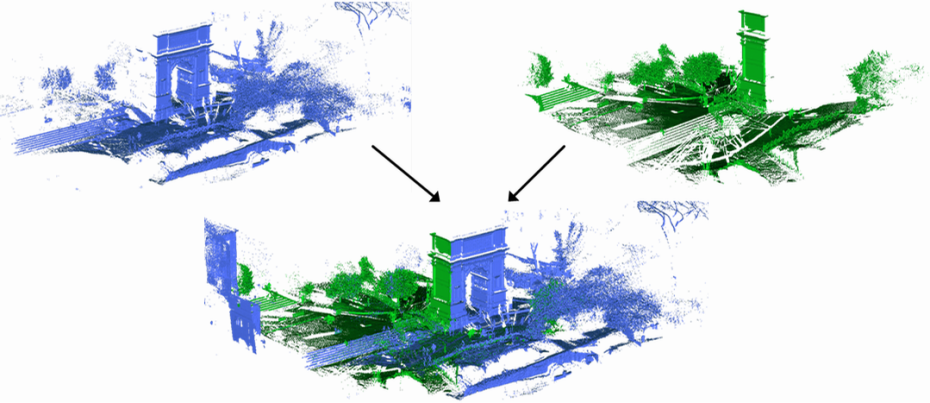
\includegraphics[width=.7\textwidth]{figs/point-cloud-registration-example.png}
  \caption[Exemplo do registro de nuvem de pontos]{Exemplo de registro de par de nuvem de pontos. As nuvens representam porções diferentes de uma mesma cena e possuem elementos 
  em comum.}
  \label{fig:point-cloud-registration-example}
\end{figure}

Com isso, ao utilizar como nuvem de pontos o mapa 
e \textit{landmarks} de cada robô e restringir que a transformação $\tr$ seja uma transformação de corpo rígido $\trr{}$, é possível determinar 
a posição 
relativa entre eles. A Transformação $\trr{}$ é definida por um ângulo
de rotação e um vetor de translação entre dois sistemas de referência:
\begin{equation}
  \trr{} = \begin{bmatrix}
    \theta & d_x & d_y 
  \end{bmatrix}^T
  \label{eq:rigid-transform}
\end{equation}

A premissa para utilizar essa técnica é que ao 
explorar o mesmo ambiente, o mapa criado por cada robô possui 
elementos (\textit{landmarks}) em comum com 
os mapas dos demais e, portanto, é possível identificar e estabelecer 
relação entre as \textit{landmarks} em comum para determinar a 
transformação $\trr{}$ que melhor as alinhem.

Porém, como a única informação que caracteriza uma \textit{landmark} é a 
sua posição no sistema de referência local, fica difícil determinar se 
ela também foi observada por outros e, portanto, está em seu mapa. Essa 
dificuldade se deve à utilização do sensor LiDAR, pois em soluções que usam 
câmeras RGB ou de RGB-D, as texturas e cores podem ser utilizadas para 
identificar pontos de interesse.

Para superar essa limitação, utilizou-se um descritor de características 
para descrever uma \textit{landmark} a partir de sua vizinhança, dessa 
forma criando uma ``impressão digital'' que se repetiria no outro mapa, 
possibilitando identificar quando uma mesma \textit{landmark} foi observada 
pelo outro par. Então foi desenvolvido um descritor de características 
inspirado no descritor \textit{Spin Image} \cite{johnson1999using} 
para o caso planar do mapa de \textit{landmarks}. A Figura \ref{fig:feature-descriptor} ilustra o descritor. Ele define uma 
vizinhança em torno da \textit{landmark} descrita e a divide em setores. 
Cada setor possui uma posição correspondente no vetor de características; 
a cada posição do vetor corresponde a quantidade de \textit{landmarks} 
vizinhas à \textit{landmark} descrita em seu setor correspondente.

\begin{figure}[h]
  \centering
  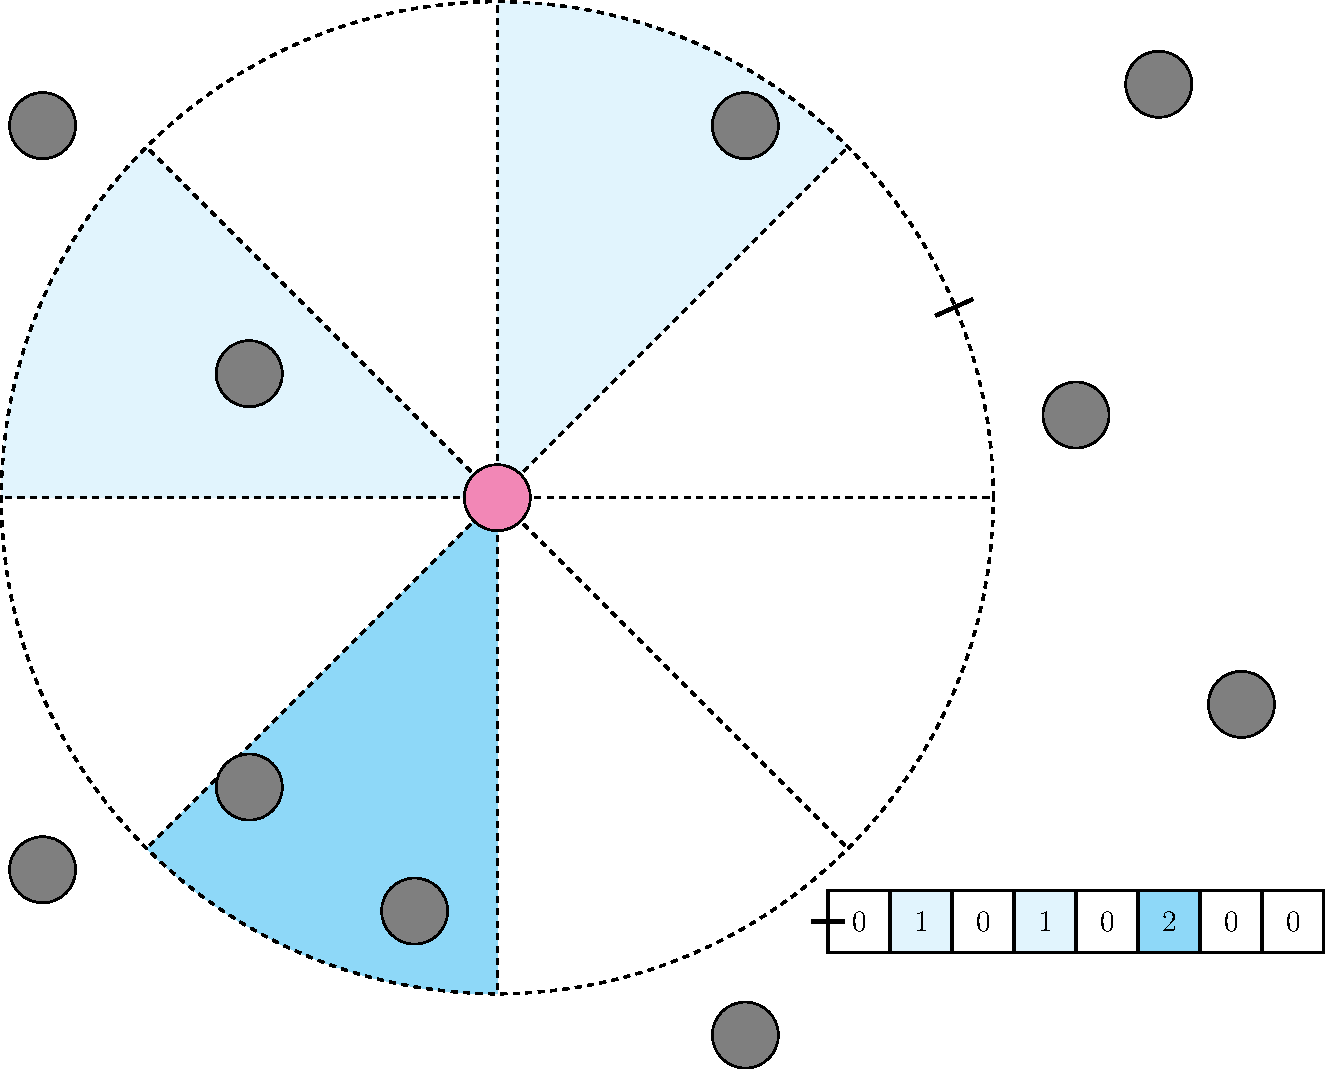
\includegraphics[width=0.6\textwidth]{figs/feature-descriptor.tex}
  \caption[Descritor de características utilizado no registro de nuvem de pontos]{Ilustração do descritor de característica utilizado para 
  relacionar \textit{landmarks} entre os mapas dos agente. As \textit{landmarks} estão representadas por círculos em cinza, a \textit{landmark} descrita é representada em magenta. O vetor descritor está representado no canto inferior direito. Cada posição do vetor corresponde a um setor da circunferência tracejada. Os setores que 
  possuem \textit{landmarks} vizinhas estão realçados em tons de azul.}
  \label{fig:feature-descriptor}
\end{figure}

Depois que o vetor de características de cada \textit{landmark} em ambos os 
mapas é criado, são estabelecidas correspondências entre pares de vetores de descrição (um de cada mapa) utilizando 
como critério a distância euclidiana. 
Então, utiliza-se o algoritmo \textit{Random Sample Consensus} (RANSAC) 
\cite{fischler1981random} para estimar a melhor transformação que alinha 
os dois mapas.

Aplicando a transformação obtida no mapa de \textit{landmarks} do outro 
robô, o primeiro avalia quantas \textit{landmarks} a transformação alinha 
corretamente, e se há alguma \textit{landmark} com alinhamento indefinido. 
Um alinhamento é tido como correto quando a distância $d$ entre as 
\textit{landmarks} é menor que um limiar $\delta_{\text{near}}$ e como 
indefinido se a distância está entre os limiares 
$\delta_{\text{near}} \leq d < \delta_{far}$. A transformação é então aceita 
como correta se não existirem alinhamentos indefinidos e a quantidade de 
alinhamentos corretos é maior ou igual a quatro.

% TODO: fazer imagem do pipeline de registro

\section{Troca de Mapas}
\label{sec:seif-map-exchange}

Dada a transformação da posição relativa entre o par de robôs $(j, k)$, 
obtida pelo registro dos mapas de \textit{landmarks} dos robôs $j$ e 
$k$, resta incorporar os mapas de um no outro. As próximas duas Seções abordam 
a fusão dos vetores e matrizes de informação de ambos os agentes, e de seus 
mapas de ocupação. Ambas as fusões exploram o caráter aditivo de suas 
respectivas representações.

\subsection{Troca do vetor e matriz de informação}
\label{sec:seif-info-exchange}
A exposição que segue abaixo nessa Seção segue de \cite[Seção~12.11]{thrun2005probabilistic}. 

Para que um robô incorpore os vetores de estado e informação e a matriz 
de informação um do outro, é necessário antes mudar o sistema de 
referência de um para o outro. Em posse da transformação de mudança do 
sistema de referência do robô $j$ para o sistema de referência do robô 
$k$, $\trr{j\to k}$, 
\begin{equation}
  \trr{j \to k} = \begin{pmatrix}
    \theta^{j\to k} & d_x^{j\to k} & d_y^{j\to k}
  \end{pmatrix}
\end{equation}
onde:
\begin{itemize}
  \item $\theta^{j\to k}$ é o ângulo de rotação necessário para alinhar 
os eixos do sistema de referência local do robô $k$ com os eixos do 
sistema de referência do robô $j$
  \item $d_x^{j\to k}$ descolamento no eixo $x$ que leva a componente $x$ 
da origem do sistema de referência do robô $k$ para a origem do 
sistema de referência do robô $j$
  \item $d_y^{j\to k}$ descolamento no eixo $y$ que leva a componente $y$ 
da origem do sistema de referência do robô $k$ para a origem do 
sistema de referência do robô $j$
\end{itemize}

A posição da \textit{i}-ésima \textit{landmark} do vetor de estados do 
robô $j$ é reescrita no sistema de referência do robô $k$ da seguinte 
forma:
\begin{equation}
  \bsubvec{m}{i}^{j\to k} = \underbrace{\begin{bmatrix}
    d_x^{j\to k}\\ d_y^{j\to k}
  \end{bmatrix}}_{\mb{\delta}_m}
  + \underbrace{\begin{bmatrix}
      \cos(\theta^{j\to k}) & \sin(\theta^{j\to k}) \\
      -\sin(\theta^{j\to k}) & \cos(\theta^{j\to k})
    \end{bmatrix}}_{\bsubvec{A}{m}}
  \begin{bmatrix}
    m_x^i \\ m_y^i
  \end{bmatrix}
\end{equation}
Já a pose do robô $j$ no sistema de referência do robô $k$ é dada por:
\begin{equation}
  \bsubvec{x}{r}^{j\to k} =  \underbrace{\begin{bmatrix}
    \theta^{j\to k} \\ d_x^{j\to k}\\ d_y^{j\to k}\\
  \end{bmatrix}}_{\mb{\delta}_r}
  + \underbrace{\begin{bmatrix}
      1 & 0 & 0\\
      0 & \cos(\theta^{j\to k}) & \sin(\theta^{j\to k})\\
      0& -\sin(\theta^{j\to k}) & \cos(\theta^{j\to k})
  \end{bmatrix}}_{\bsubvec{A}{r}}
  \begin{bmatrix}
    \theta^j\\ x^j \\ y^j
  \end{bmatrix} 
\end{equation}

Definindo o vetor $\bvec{\Delta}$ e a matrix $\bvec{A}$ como:
\begin{equation}
  \bvec{\Delta} = \begin{bmatrix}
    \mb{\delta}_r & \mb{\delta}_m & \hdots & \mb{\delta}_m
  \end{bmatrix}^T
\end{equation}
e
\begin{equation}
  \bvec{A} = \begin{bmatrix}
    \bsubvec{A}{r} & \bvec{0} & \hdots & \bvec{0} \\
    \bvec{0} & \bsubvec{A}{m} & \hdots & \bvec{0}\\
    \vdots & \vdots & \ddots & \vdots\\
    \bvec{0} & \bvec{0} & \hdots & \bsubvec{A}{m}
  \end{bmatrix}
\end{equation}
pode-se reescrever a mudança de referência do vetor de estados do robô 
$j$ para o sistema de referência do robô $k$, como:
\begin{equation}
  \bvec{x}^{j\to k} = \bvec{\Delta} + \bvec{A} \, \bvec{x}^j
  \label{eq:state-vector-change-reference-frame}
\end{equation}

Com o resultado, a mudança de sistema de referência do robô $j$ para o 
do robô $k$, mostrado na Equação 
\ref{eq:state-vector-change-reference-frame}, e usando como hipótese 
que não há ganho ou perda de informação ao mudar o sistema de referência 
dos vetores e matrizes do robô $j$ para o robô $k$, ou seja que
\begin{equation}
  \pr{\bsubvec{x}{t}^{j\to k} \given \bsubvec{z}{1:t} , \bsubvec{u}{1:t}}
  = \pr{\bsubvec{x}{t}^j \given \bsubvec{z}{1:t} , \bsubvec{u}{1:t}}
  \label{eq:map-exchange-equivalence}
\end{equation}
chegamos aos valores de $\infov{}^{j\to k}$ (vetor de informação) e 
$\infom{}^{j\to k}$ (matriz de informação) através do seguinte 
desenvolvimento:
\begin{equation}
  \begin{aligned}
    \pr{\bsubvec{x}{t}^{j\to k} \given \bsubvec{z}{1:t} , \bsubvec{u}{1:t}} &= \eta \exp\parentheses{-\frac{1}{2} 
  \parentheses{\bupvec{x}{j\to k}}^T \infom{}^{j\to k} \,\bvec{x}^{j\to k} + \parentheses{\bvec{x}^{j\to k}}^T \infov{}^{j\to k}}\\
  &= \eta \exp\parentheses{-\frac{1}{2} 
  \parentheses{\bvec{\Delta} + \bvec{A} \, \bvec{x}^j}^T \infom{}^{j\to k} \,\parentheses{\bvec{\Delta} + \bvec{A} \, \bvec{x}^j} + \parentheses{\bvec{\Delta} + \bvec{A} \, \bvec{x}^j}^T \infov{}^{j\to k}}\\
  &= \begin{split}
  \blue{\eta} \exp \Biggl( &\blue{\underbrace{-\frac{1}{2} \bvecT{\Delta}\infom{}^{j\to k} \bvec{\Delta}}_{\text{constante}}} - \frac{1}{2}\bvecT{\Delta}\infom{}^{j\to k}\bvec{A}\bupvec{x}{j} - \frac{1}{2}\bupvecT{x}{j}\bvecT{A}\infom{}^{j\to k}\bvec{\Delta} \\
    & -\frac{1}{2} \bupvecT{x}{j}\bvecT{A}\infom{}^{j\to k}\bvec{A}\bupvec{x}{j} + \blue{\underbrace{\bvecT{\Delta}\infov{}^{j\to k}}_{\text{constante}}} + \bupvecT{x}{j}\bvecT{A}\infov{}^{j\to k} \Biggr)
  \end{split}\\
  &= \blue{\eta}\exp\parentheses{-\frac{1}{2}\bupvecT{x}{j}\parentheses{
    \bvecT{A} \infom{}^{j\to k} \bvec{A}}\bupvec{x}{j} - \bupvecT{x}{j}\bvecT{A}\infom{}^{j\to k}\bvec{\Delta} + \bupvecT{x}{j}\bvecT{A}\infov{}^{j\to k}}\\
  &= \begin{split}
    \blue{\eta}\exp\Biggl(-\frac{1}{2}&\bupvecT{x}{j}\underbrace{\parentheses{
    \bvecT{A} \infom{}^{j\to k} \bvec{A}}}_{\infom{}^j}\bupvec{x}{j}\\
    &+ \bupvecT{x}{j}\bigl(\underbrace{-\bvecT{A}\infom{}^{j\to k}\bvec{\Delta} + \bvecT{A}\infov{}^{j\to k}}_{\infov{}^j}\bigr)\Biggr)
  \end{split}
  \end{aligned}
\end{equation} 

Utilizando a equivalência da Equação \ref{eq:map-exchange-equivalence}, 
têm-se:
\begin{align}
  \infom{}^j &= \bvecT{A} \infom{}^{j\to k} \bvec{A}\\
  \infov{}^j &= -\bvecT{A}\infom{}^{j\to k}\bvec{\Delta} + \bvecT{A}\infov{}^{j\to k}
\end{align}
e como $\bvec{A}$ é ortogonal ($\bvec{A}^{-1} = \bvecT{A}$), temos que 
$\infov{}^{j\to k}$ e $\infom{}^{j\to k}$ são obtidos da seguinte forma:
\begin{align}
  \infom{}^{j\to k} &= \bvec{A}\infom{}^j \bvecT{A}
  \label{eq:infom-transformed}\\
  \infov{}^{j\to k} &= \bvec{A} \parentheses{\infov{}^j +  
  \infom{}^j\bvecT{A}\bvec{\Delta}}
  \label{eq:infov-transformed}
\end{align}

Com o vetor de informação e a matriz de informação do 
robô $j$ reescritos no sistema de referência do robô $k$, Equações \ref{eq:infov-transformed} e \ref{eq:infom-transformed} respectivamente, criamos as seguintes grandezas aumentadas:
\begin{align}
  \infov{t}^* &= \begin{bmatrix}
    \brac{\infov{t}^k}^T & \brac{\infov{t}^{j\to k}}^T
  \end{bmatrix}^T\\
  \infom{t}^* &= \begin{bmatrix}
    \infom{t}^k & \bvec{0}\\
    \bvec{0} & \infom{t}^{j\to k}
  \end{bmatrix} 
\end{align}

O vetor e a matriz de informação aumentados são simplesmente o vetor e matriz do robô $k$ concatenados com o 
vetor e matriz de informação do robô $j$ transformados para o sistema 
de referência do robô $k$. Portanto, há mais de uma linha/bloco que 
possui informação relacionada a uma mesma \textit{landmark} que foi observada 
por ambos os robôs separadamente, então resta ainda fundir linhas e 
blocos que dizem respeito à mesma \textit{landmark}. Para isso, basta 
somá-los; no exemplo abaixo, supõe-se que os blocos 2 e 4 do vetor e 
matriz de informação correspondem ao mesmo objeto:
\begin{align}
  \begin{bmatrix}
    \infom{11} & \infom{12} & \infom{13} & \infom{14}\\
    \infom{21} & \infom{22} & \infom{23} & \infom{24}\\
    \infom{31} & \infom{32} & \infom{33} & \infom{34}\\
    \infom{41} & \infom{42} & \infom{43} & \infom{44}
  \end{bmatrix} &\rightarrow \begin{bmatrix}
    \infom{11} & \infom{12} + \infom{14} & \infom{13}\\
    \infom{21}+\infom{41} & \infom{22}+\infom{42} + \infom{24}+\infom{44} & \infom{23}+\infom{43} \\
    \infom{31} & \infom{32} + \infom{34} & \infom{33} \\
  \end{bmatrix}
  \label{eq:info-matrix-fusion}\\
  \begin{bmatrix}
    \infov{1} \\ \infov{2} \\ \infov{3} \\ \infov{4}
  \end{bmatrix} &\rightarrow \begin{bmatrix}
    \infov{1} \\ \infov{2} + \infov{4} \\ \infov{3}
  \end{bmatrix}
\end{align}

Por último, depois da fusão dos blocos da matriz e do vetor de 
informação, é necessário ajustar os elementos correspondentes do vetor 
média. Para isso foi utilizado o método descrito no Algoritmo \ref{alg:seif-slam-mean-recovery}, mas ao invés da otimização ser realizada 
num conjunto de \textit{landmarks} observadas, ela é realizada 
no conjunto 
de \textit{landmarks} que foram observadas por ambos os robôs do par e,
portanto, tiveram seus elementos fundidos.

\subsection{Troca de grades de ocupação}
Similarmente a troca do vetor e matriz de informação, as células da 
grade de ocupação de um robô são projetadas na do outro por meio da 
transformação $\trr{j \to k}$. O logaritmo da razão de chance da \textit{i}-ésima célula da grade de ocupação do robô $k$ é atualizada da 
seguinte forma:
\begin{equation}
  l_i^k = l_i^{j\to k} + l_i^k - l_0^k
\end{equation}

A Figura \ref{fig:grid-map-exchange} ilustra a fusão das grades de 
ocupação de um par de robôs. É possível observar que um robô passa a ter 
informações de células que não podem ser observadas do seu ponto de 
vista, mas que foram observadas pelo outro robô.

\begin{figure}[]
  \centering
  \begin{subfigure}{0.45\textwidth}
    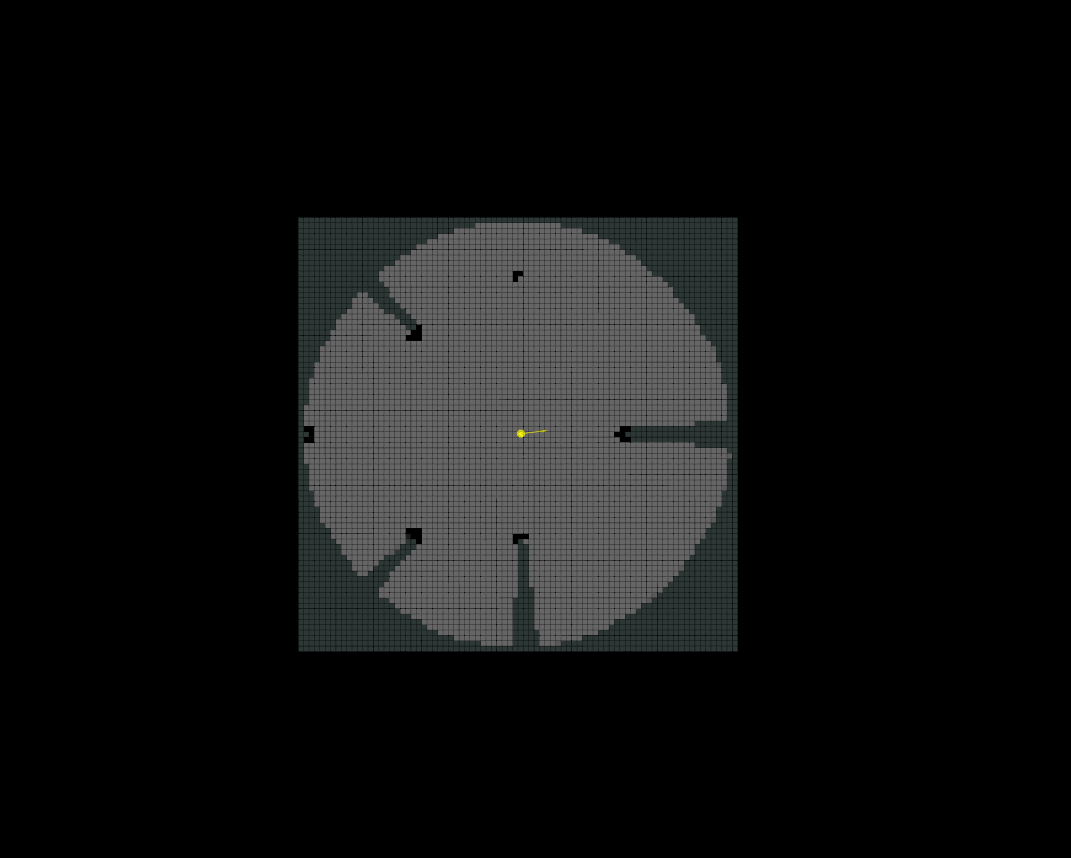
\includegraphics[width=\textwidth]{figs/grid-rb1.png}
    \caption{Mapa de grade do robô 1. O robô está no centro da grade 
      em amarelo.}
    % \label{fig:}
  \end{subfigure}
  \hfill
  \begin{subfigure}{0.45\textwidth}
    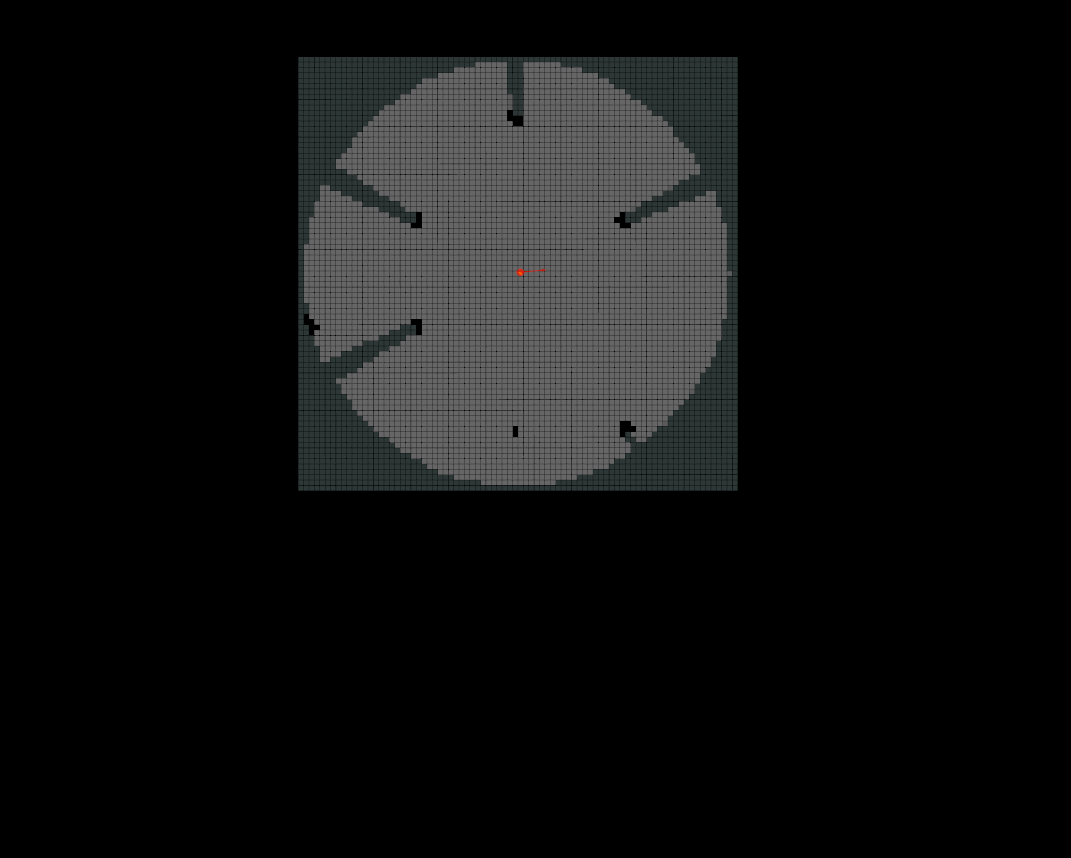
\includegraphics[width=\textwidth]{figs/grid-rb2.png}
    \caption{Mapa de grande do robô 2. O robô está no centro da grade 
      em vermelho.}
    % \label{fig:}
  \end{subfigure}
  \begin{subfigure}{0.65\textwidth}
    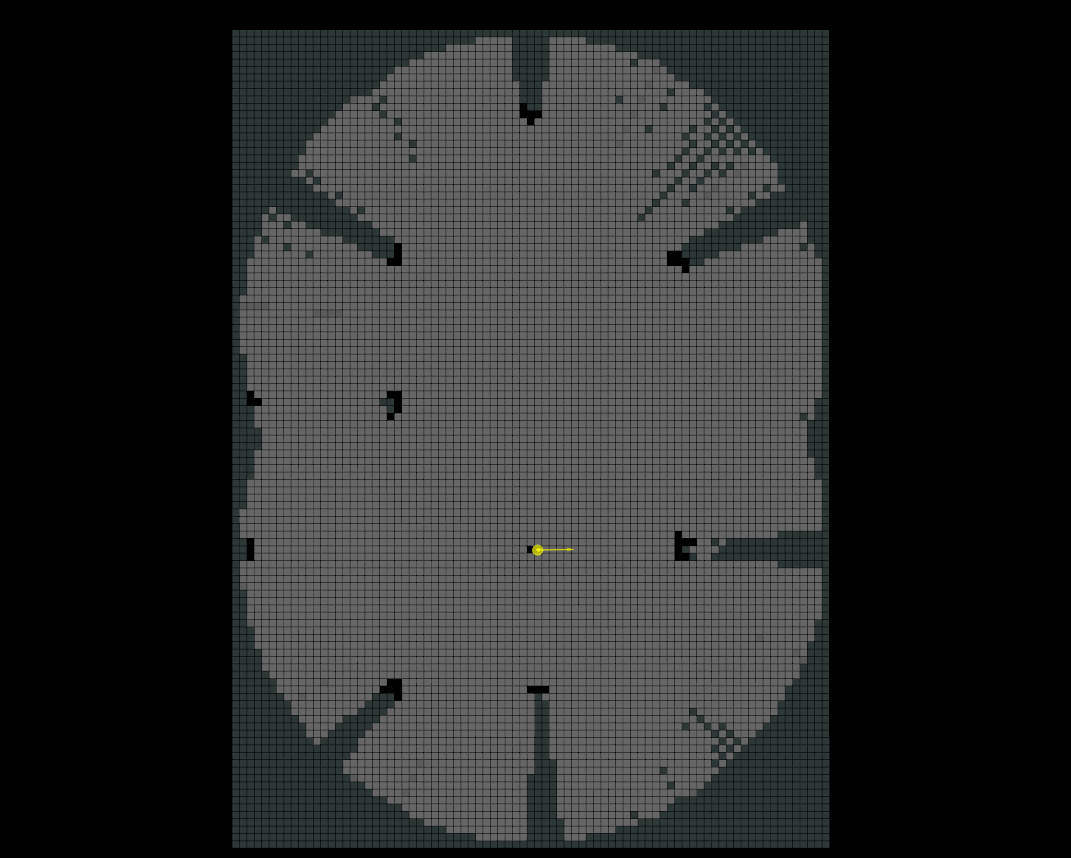
\includegraphics[width=\textwidth]{figs/map-merge.png}
    \caption{Mapa de grade do robô 1 após incorporar o mapa de grade 
      do robô 2. }
    % \label{fig:}
  \end{subfigure}
  \caption[Fusão de mapas de grade de ocupação]{As imagens menores representam os mapas de grade 
  individuais de cada robô. A imagem maior representa o mapa de grade do
  primeiro robô após receber o mapa de grade do segundo. Note que algumas
  células com probabilidade de ocupação 0.5 (nem ocupada e nem desocupada) pelo robô 1 passam a ter probabilidade de ocupação diferente de 0.5, pois são observadas do ponto de vista do robô 2.}
  \label{fig:grid-map-exchange}
\end{figure}
